% preamble

\documentclass{article}
%% \usepackage{times}
\usepackage{latexsym}
\usepackage{graphicx}
\usepackage{url}
\usepackage{hyperref}
\usepackage{listings}
\hypersetup{colorlinks=true}


\begin{document}

% top matter

\title{Dictionary Application, Summer 2017}
\author{Oprea Denisa}
\date{\today}
\maketitle

\begin{tabbing}
\\ \\ \\ \\ \\ \\ \\ \\ \\ \\ \\ \\ \\ \\ \\ \\ \\ \\ \\ \\ \\ \\ \\ \\
\end{tabbing}

\begin{tabbing}
\indent{Teachers:}  \=\ {Costin B\u{a}dic\u{a} and Alex Becheru} \\
\indent{Section:}   \=\  {Computers with teaching in Romanian Class} \\
\indent{Group:}      \>  C.R. 1.2.  \\
\indent{Year of study:} \=\ {I}

\end{tabbing}

\pagebreak
% sections
\section{Problem statement}
\ \ \ \ Write a dictionary application. The dictionary should allow for inserting a word, updating the de?nition of an existing word and looking up de?nition of a word. Note that a word may have multiple de?nitions attached to it. The dictionary should use ?les for storing and loading its data. 


\section{Pseudocode}


\lstset{
  language=C,                % choose the language of the code
  numbers=left,                   % where to put the line-numbers
  stepnumber=1,                   % the step between two line-numbers.        
  numbersep=5pt,                  % how far the line-numbers are from the code
  backgroundcolor=\color{white},  % choose the background color. You must add \usepackage{color}
  showspaces=false,               % show spaces adding particular underscores
  showstringspaces=false,         % underline spaces within strings
  showtabs=false,                 % show tabs within strings adding particular underscores
  tabsize=4,                      % sets default tabsize to 2 spaces
  captionpos=b,                   % sets the caption-position to bottom
  breaklines=true,                % sets automatic line breaking
  breakatwhitespace=true,         % sets if automatic breaks should only happen at whitespace \lstinputlisting;
}

\begin{lstlisting}

add_word (struct dictionary *dictionary, char word[100]) {

    struct dictionary *iterator = dictionary;
    struct dictionary *newWord = malloc (sizeof (struct dictionary));
    char yon;
    char definition[100];

    while (iterator->nextWord != NULL) {
        if (strcmp (iterator->nextWord, word) == 0) {
            printf("\nWord already exists.");
            return;
        }
        iterator = iterator->nextWord;
    }

    iterator->nextWord = newWord;
    newWord->nextWord = NULL;
    strcpy(newWord->word, word);
    printf("\nYou've added a new word \"%s\" do you want to add a definition(Y/N)? ", word);
    yon = getch();
    if (yon == 'n' || yon == 'N')
        return;
    printf("\nEnter the word first definition: ");
    scanf("%s", &definition);
    strcpy(newWord->definition[0], definition);

}


 add_definition (struct dictionary *dictionary, char word[100], char definition[100]) {

    int i;
    struct dictionary *iterator = dictionary;

    while (iterator->nextWord != NULL) {
        if (strcmp (iterator->nextWord->word, word) == 0) {
            for (i = 0; strlen(iterator->nextWord->definition[i]) != 0; i++);
            strcpy(iterator->nextWord->definition[i], definition);
            printf("\nDefinition added successfully.");
            return;
        }
        iterator = iterator->nextWord;
    }
    printf("\nGiven word does not exists in dictionary.");
}


void save_to_file(struct dictionary *dictionary){




    FILE *f = fopen("dictionary.txt", "a+");

    if (f == NULL)
    {
        printf("\nError saving to file!");
        return;
    }

    int i;
    struct dictionary *iterator = dictionary;

	while (iterator->nextWord != NULL) {
		fprintf(f, "\n\nWord: %s", iterator->nextWord->word);
		for (i = 0; strlen(iterator->nextWord->definition[i]) != 0; i++)
			fprintf(f, "\nDefinition %d: %s", i + 1, iterator->nextWord->definition[i]);
		fprintf(f, "\n");
		iterator = iterator->nextWord;
	}
	fclose(f);

	printf("\nYour content has been saved to file \"%s\".", "dictionary.txt");
}


\end{lstlisting}


\begin{center}
\begin{tabbing}

\end{tabbing}
\end{center}



\subsection{Pseudocode description}
\textbf{}
\indent The {\bf add\_word} function is for adding a new word to our dictionary. It accepts 1 parameter, the name of the word we will add. 

\indent The {\bf add\_definition} function is for adding a new definition to an existing word. 

\indent The {\bf save\_to\_file} is for saving the current dictionary to a file.


\section{Application Design}
\subsection{Main}
\textbf{}
\indent The {\bf main} of my program contains a {\bf while} loop so the user will be forced to choose a valid option. He has the option to choose from ten different options.


\subsection{Input Data}
\textbf{}
\indent For my program, input data are "decision", "decision\_1", "decision\_2", "decision\_3"."decision" is the choice that you have to make in order to choose an option from the menu and in some cases will be overwritten with something else, "decision\_1" is used for telling the word that will be added or the word we search for. "decision\_2" variable is used to tell the definition we will add or the definition we search for. "decision\_3" is used to tell the new definition in order to change an old one.

\subsection{Output Data}
\textbf{}
\indent The data outputs resulted from functions processing. The functions include adding, deleting, changing a word or a definition from our dictionary.




\pagebreak

\subsection{Functions used}
\textbf{}
\indent{\bf void add\_word (struct dictionary *dictionary, char word[100])} function is for adding a new word to our dictionary. If the user want he can immediately add a new definition.  

{\bf void add\_definition (struct dictionary *dictionary, char word[100], char definition[100])} function is for adding a new definition to an existing word. 

{\bf void change\_word (struct dictionary *dictionary, char word[100], char new\_word[100])} function is used to find the given word and replace it with the one user specified.

{\bf void change\_definition (struct dictionary *dictionary, char word[100], char definition[100], char new\_definition[100])} function is used to find the given word and definition, will replace definition with the one user specified.

{\bf void show\_all\_words (struct dictionary *dictionary)}, function is used to print all words and their definitions to the console.

{\bf void show\_all\_definitions (struct dictionary *dictionary, char word[100])} function is used to print all definitions of a given word to the console.

{\bf void delete\_word (struct dictionary *dictionary, char word[100])} function is used to delete a given word from the dictionary.

{\bf void delete\_definition (struct dictionary *dictionary, char word[100], char definition[100])} function is used to delete a given definition of a given word.



{\bf void save\_to\_file (struct dictionary *dictionary)} is for saving the current dictionary to a file under the same folder.  

\section{Source code}
\textbf{}
\indent My program is called "Dictionary Application". It is created in C99 standard.

The code is compiled with the following compiler: "GNU GCC Compiler"



\section{Experiments and results}
\subsection{GCC Compiler}
\textbf{}
\indent For GCC compiler here are the results of running the application.

It runs as follow: \\ \\
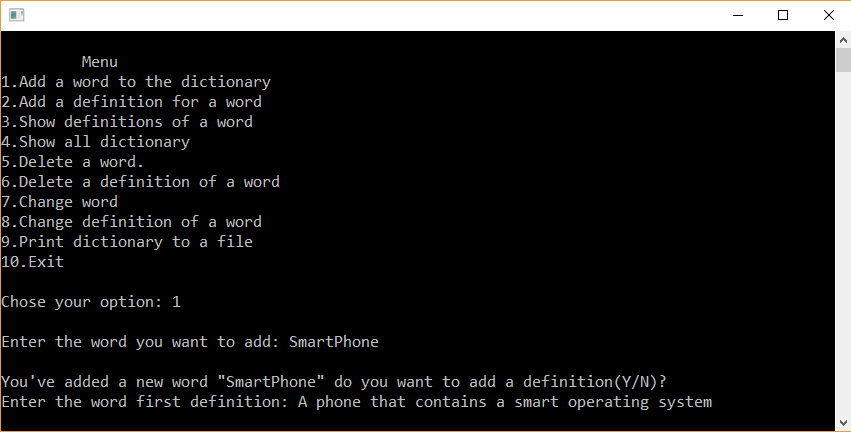
\includegraphics[scale=1]{e1} \\
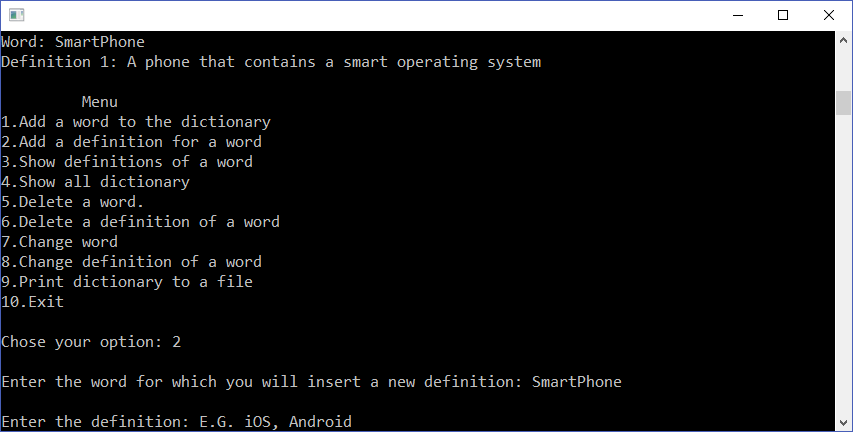
\includegraphics[scale=1]{e2} \\ \\
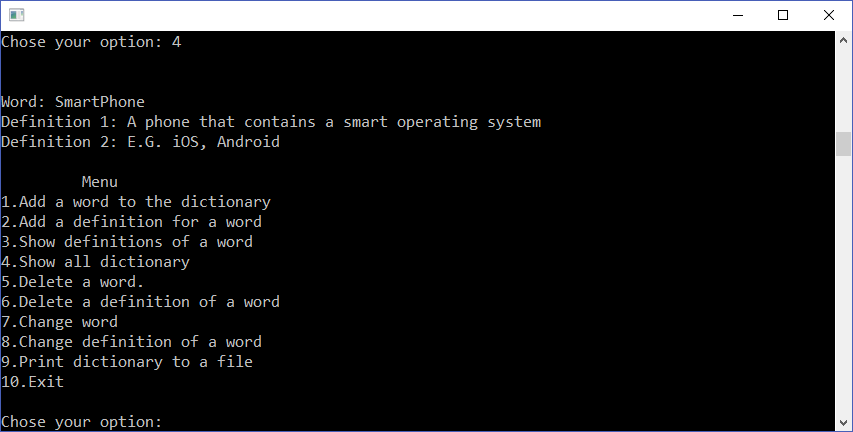
\includegraphics[scale=1]{e3} \\
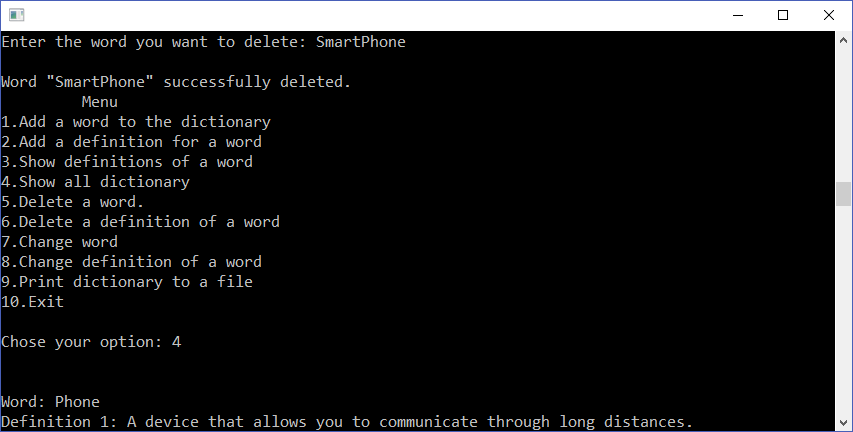
\includegraphics[scale=1]{e4} \\ \\
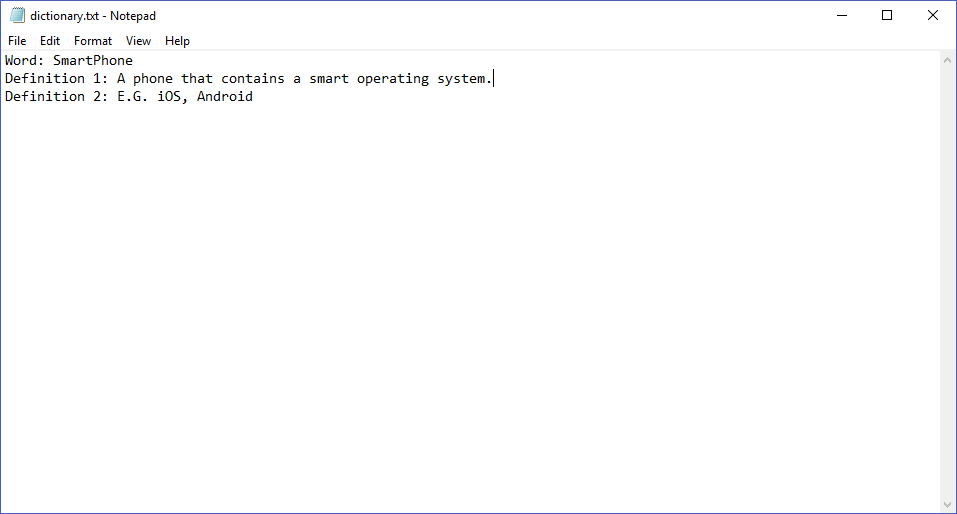
\includegraphics[scale=1]{e5}

\pagebreak

\section{Conclusions}
\textbf{}
\indent Using linked list was a great because of the performance. Code is simple and easy to understand because i used linked lists instead of matrices.


% bibliography
\begin{thebibliography}{9}

    \bibitem{wiki}
     {\bf Robert I. Pitts} \\
     \url{https://www.cs.bu.edu/teaching/cpp/string/array-vs-ptr/}


\end{thebibliography}

\end{document}